\chapter{BIODATA PENULIS}

\begin{wrapfigure}{l}{0.3\textwidth}
	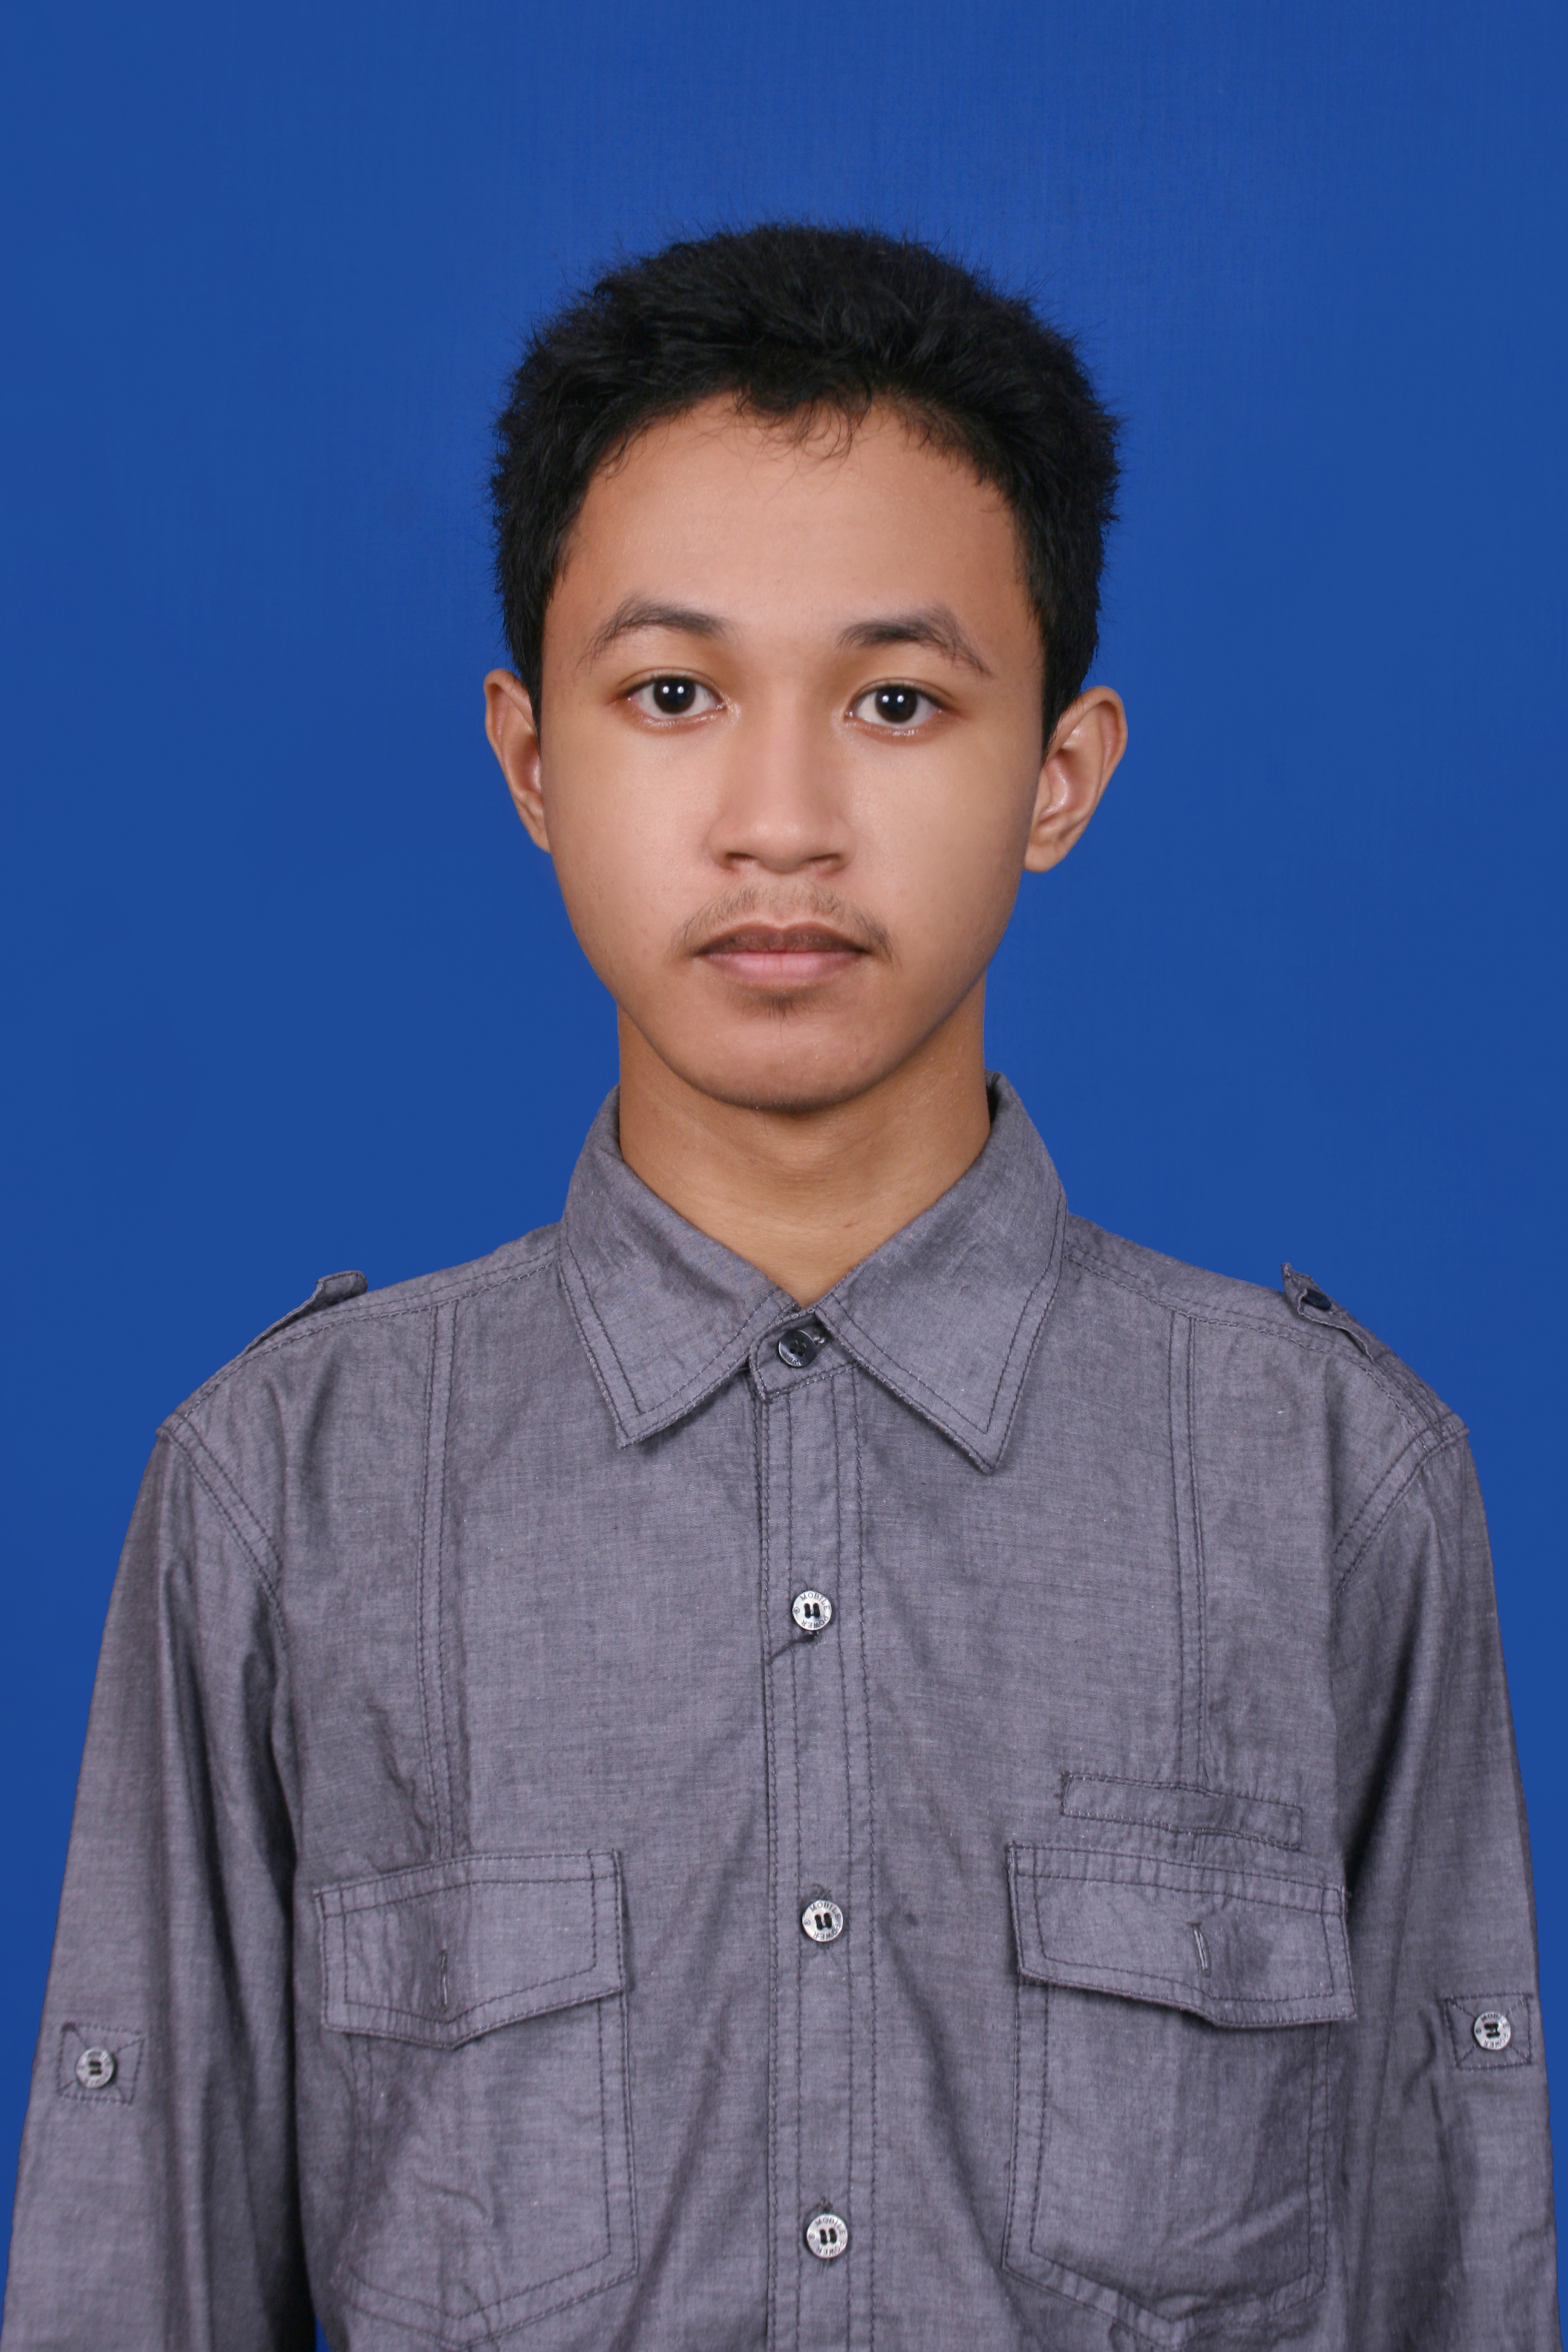
\includegraphics[height=0.3\textheight]{penutup/img/IMG_3563}
\end{wrapfigure}

Penulis bernama Muhammad Ghazian, putra ketiga dari empat bersaudara yang lahir pada tanggal 29 Desember 1995 di Bogor. Penulis telah mengenyam pendidikan di Sekolah Dasar Islam Terpadu Ummul Quro pada tahun 2002 hingga 2008, Sekolah Menengah Pertama Negeri 1 Bogor pada tahun 2008 hingga 2011, dan Sekolah Menengah Atas Neger 2 Bogor pada tahun 2011 hingga 2014. Pada masa penulisan, penulis sedang menempuh masa studi S1 di Institut Teknologi Sepuluh Nopember, Surabaya di \jurusanlama.

Selama masa studi, penulis memiliki ketertarikan yang dalam mengenai \textit{Artificial Intelligence}, rancang bangun aplikasi \textit{game}, dan rancang bangun aplikasi sistem informasi. Keinginan penulis dalam mengajar juga mendorong penulis menjadi asisten dosen pada mata kuliah Dasar Pemrograman, Struktur Data, Perancangan dan Analisis Algoritma (I), dan Perancangan dan Analisis Algoritma (II). Karya penulis semasa perkuliahan diantaranya adalah pembangunan Sistem Penilaian Unit Angka Kredit Guru untuk Kementerian Pendidikan Provinsi Jawa Timur. Selain itu, penulis juga cukup aktif membuat \textit{game} di sela-sela waktu kosong.

Di luar kesibukan akademik, penulis cukup aktif di lembaga dakwah jurusan sebagai salah satu staf. Penulis juga berkontribusi dalam berbagai kepanitiaan, baik dalam skala kecil (yaitu dalam kampus) maupun skala nasional. Kegiatan terakhir penulis adalah membantu kegiatan pelatihan nasional bagi peserta Olimpiade Komputer Indonesia pada Februari dan Maret 2018 lalu.

